\documentclass[11pt]{amsbook}

\usepackage[turkish]{babel}
\usepackage{../Ceyhun}
\usepackage{../amsTurkish}

 
\begin{document}

 
 
\chapter{}
\vspace{-3cm}\hPage{Ceyhun/101}
\begin{figure}[h]
    \centering
    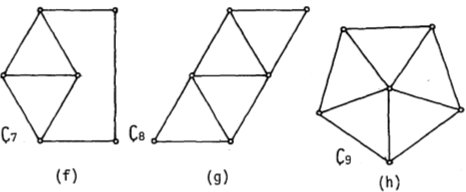
\includegraphics{ceyhun-101-fig04-jpg}
    \caption{  Ayrıt çizgesinde bulunamayacak irgitilmiş altçizgel er. }
    \label{fig:my_label}
\end{figure}
\vspace{-2cm}
\begin{theorem}
    \begin{tabular}{p{5cm}}
        \vspace{2cm}\textup{de} tek üçgenden \textup{anladığımız, eğer Ç(d,a) daki bir üçgen altçizgenin ( D(3) ) teksayıdaki düğümlerine bitiş olan bir düğüm varsa D(3)} tek üçgen, \textup{başkaca durumlarda D(3)} çift üçgendir.
    \end{tabular} 
\end{theorem}
 
 
 
\begin{definition} 
    \begin{tabular} {p{5cm}}
        \vspace{1cm}$Ç(d,a)$ daki her ayrıtı n sayıda dizi bağlı ayrıtla değiştirerek elde edilen ve Ç(d,a)_{+n} \linebreak  biçiminde gösterilen çizgeye, Ç(d,a) nın     \textup{n-katlılı çizgesi} denir. 
    \end{tabular}
\end{definition}
  
 
  
\begin{definition}
    \begin{tabular} {p{5cm}}
         
         \vspace{20pt}A\{Ç(d,a)_{+n}} biçiminde gösterilen, Ç(d,a)_{+n} nın. n ayrıt çizgesine, Ç(d,a)nın n-katkılı \linebreak \underline{ayrıt çizgesi}  denir
    \end{tabular}
\end{definition}
      
 
\end{document}
 
 